\documentclass{IEEEcsmag}


\usepackage[colorlinks,urlcolor=blue,linkcolor=blue,citecolor=blue]{hyperref}

\usepackage{upmath}

\jvol{XX}
\jnum{XX}
\paper{8}
\jmonth{May/June}
\jname{IT Professional}
\pubyear{2021}

\newtheorem{theorem}{Theorem}
\newtheorem{lemma}{Lemma}


\setcounter{secnumdepth}{0}

\graphicspath{{pics/}}

\hyphenation{Para-View}

\usepackage{color}
\newcommand*{\fix}[1]{\textbf{\emph{\textcolor{red}{#1}}}}

\usepackage{subcaption}

\usepackage{xspace}

\newcommand*{\colormap}[1]{\textsl{#1}\xspace}
\newcommand*{\huewheel}{\colormap{Hue Wheel}}
\newcommand*{\coolwarm}{\colormap{Cool to Warm}}
\newcommand*{\blueorange}{\colormap{Blue-Orange Diverging}}
\newcommand*{\fast}{\colormap{Fast}}
\newcommand*{\turbo}{\colormap{Turbo}}

\begin{document}

\sptitle{DEPARTMENT: Visualization Viewpoints}

\title{A New Default Colormap for ParaView}

\author{Francesca Samsel}
\affil{Texas Advanced Computing Center, University of Texas at Austin, Austin, TX, 78759, USA}

\author{W. Alan Scott}
\affil{Sandia National Laboratories, Albuquerque, NM, 87123, USA}

\author{Kenneth Moreland}
\affil{Oak Ridge National Laboratory, Oak Ridge, TN, 37831, USA}

\markboth{Theresa-Marie Rhyne}{Theresa-Marie Rhyne}



\begin{abstract}
%\looseness-1
ParaView is one of the most prominent software tools for scientific visualization used by scientists around the world.
Color is a primary conduit to visually map data to its representation and thus enable investigation and interpretation of the data.
Colormap selection has a significant impact on the data revealed; its design and selection is a critical aspect of scientific data visualization.
The most common choice for a user is the program's default colormap, so careful consideration of this default is consequential.
Although the current default colormap in ParaView, a succession of colors from cool to warm, has served the community well, research shows that more nuanced colormap configurations increase discrinimability while maintaining the other critical metrics. 
This inspires us to revisit and update the default colors in ParaView.
Here we present a new ParaView default colormap, the criteria and methods of development, and example visualizations and analytic metrics.
\end{abstract}

\maketitle

\chapteri{T}he colormap is a critical part of any pseudocolor visualization.
A colormap is a simple function that maps numbers to colors, which can then be applied to visually represent a continuous distribution of values over a surface or volume.

The colormap is most recognizable to users as a bar painted with a transition of colors representing a range of numbers from low to high.

When presented with these colors, a viewer makes the reverse translation from colors back to numbers, and the efficacy of a pseudocolor visualization depends on a person's ability to perceive and translate these colors. A typical user is unlikely to be a color expert, so it is imperative that the visualization system make good choices. It is particularly important to have a good default colormap that is used in the absence of any further configuration. Many users will have neither the inclination nor the proficiency to change the default colors selected by the visualization system.

% Commenting out this figure. It shows the same thing as Figure \ref{wind3} but worse. It is also never referenced (used) in the paper. (Ken)
%% \begin{figure}[t]
%% \centerline{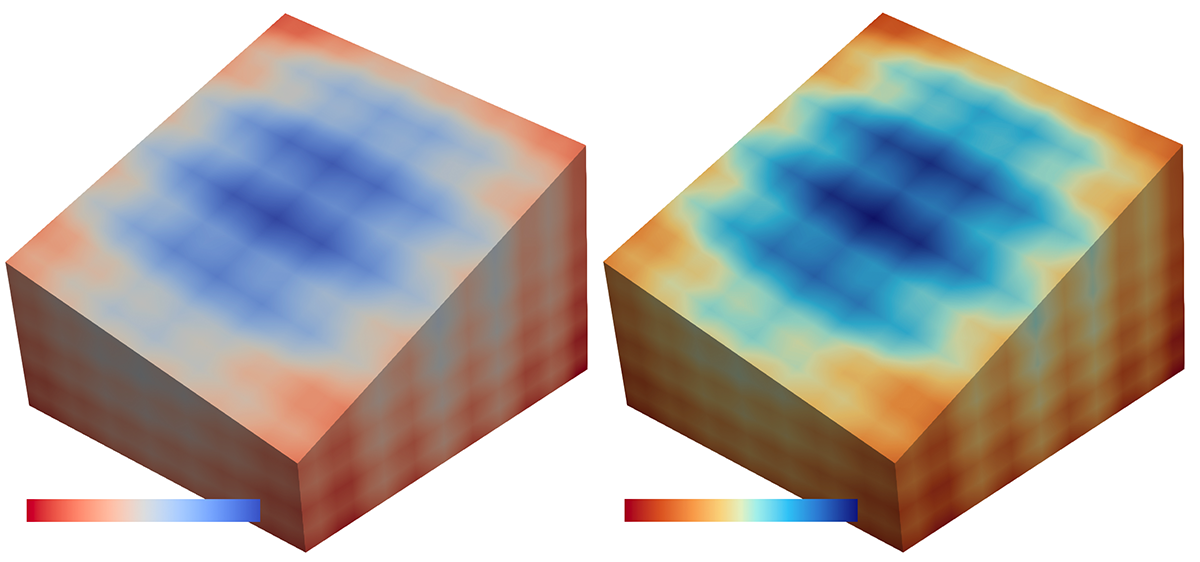
\includegraphics[width=18.5 pc]{pics/2waves.png}}
%% \caption{ParaView default colormap \coolwarm and new ParaView default colormap \fast.}
%% \label{2wave}
%% \end{figure}
  
\begin{figure*}[htb]
\centering
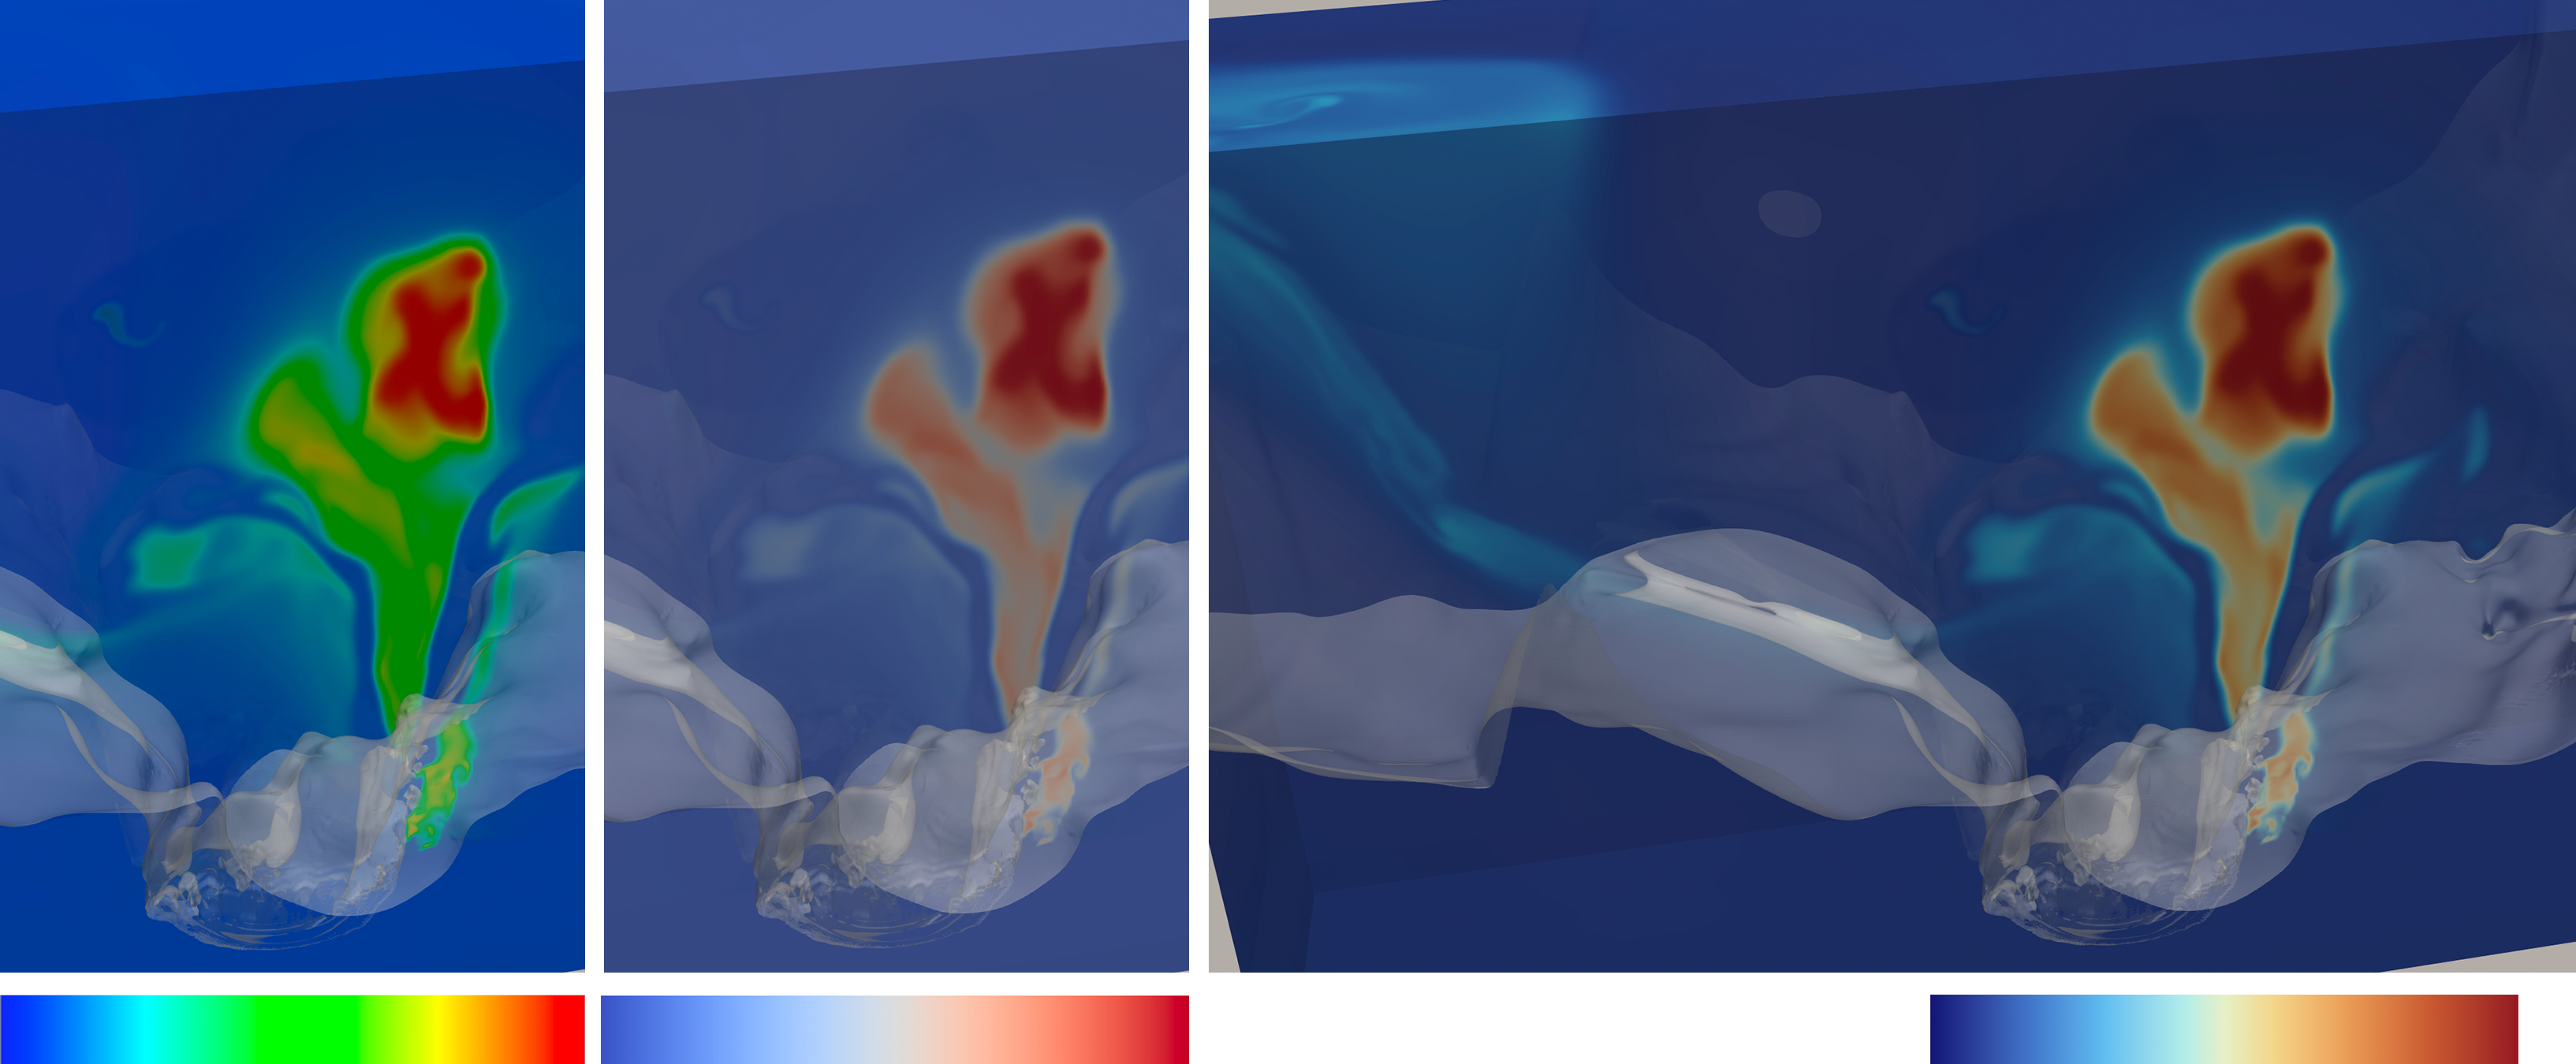
\includegraphics[width=\textwidth]{pics/Ast5.png}
\caption{
  The progression of default colormaps in ParaView.
  At left is the original (and much maligned) \huewheel colormap, which was replaced with the \coolwarm colormap many years ago.
  At right is our new \fast colormap.
  All three colormaps are demonstrated on asteroid-ocean impact temperature data with an isosurface at impact elevation.
  %The new \fast colormap, which is replacing the current default \coolwarm to colormap, on asteroid-ocean impact temperature data with an isosurface at impact elevation.
}
\label{Ast}
\end{figure*}


The authors of this paper are longtime contributors to the ParaView scientific visualization application~\cite{Ahrens2005}.
ParaView is a general-purpose tool that is used across many scientific domains and that often applies colors in a virtual 3D space.
These properties raise unique challenges for color choices in ParaView and similar products.
Care has been taken to choose colors in ParaView that work well in a variety of contexts.
This paper describes the criteria and rationale behind the default color choices in ParaView, focusing on the most recent changes to the application.
These changes arise from over 10 years working with scientists at Los Alamos National Laboratory, Sandia National Laboratories, and other institutions.


Early versions of ParaView used the \huewheel, shown in the left of Figure~\ref{Ast}, as the default colormap.
This colormap is formed by interpolating along the hues, typically from blue to red, in the HSV color space.
(Note that this colormap is often referred to as the ``Rainbow'' colormap, but we avoid that name to remove confusion with other maps designed with colors from the rainbow.)
\huewheel is a common choice as it is the simplest way to produce a sequence of many vibrant colors.
However, because these colors are defined by the physics of display technology rather than the physiology of vision, the colors are unevenly distributed and can cause features to be inappropriately accentuated or diminished.
Although the criticisms of the \huewheel colormap were known even at the inception of the ParaView software~\cite{Rogowitz1998}, there were few practical alternatives.

It was when Borland and Taylor~\cite{Borland2007} admonished ParaView by name that the developers became motivated to improve their default colormap design.
After adapting the best recommendations available at the time and drawing inspiration from the GIS community, which had extensive color map recommendations~\cite{Brewer2003}, the team settled on a \coolwarm colormap design~\cite{Moreland2009} shown in the center of Figure~\ref{Ast}.
This map adopts a diverging colormap approach with a smoothed luminance profile in the transition between hues. 

Since the introduction of the \coolwarm colormap as the default in ParaView, many practitioners have proposed alternate maps~\cite{Samsel2015}, and multiple perceptual studies have been conducted to evaluate these colormaps~\cite{Ware2017}.
Some show that the \coolwarm colormap performs less well than its alternatives, particularly with respect to its discriminability~\cite{Ware2017,Ware2019}.
Consequently, the ParaView development team has been motivated to revisit its default colormap and potentially change it.

This paper describes the processes we undertook to design a new default colormap for ParaView, which we dub ``\fast.''
Use of this colormap  can be seen in the right hand side of Figure \ref{Ast}.
We describe the criteria we used in designing this colormap, go through the process of iteratively refining colors to get us to our final map, get feedback from current users of the software, and use perceptual models to make final refinements.


\section{CRITERIA}

There are many guidelines for colormaps proposed in the literature. We use the collection compiled by Bujack et al.~\cite{Bujack2018} as a guide. The characteristics most important to us, in no particular order, are as follows.

\begin{itemize}
    
\item \emph{Discriminative powers} --
  We wish to maximize the number of just noticeable differences in the colormap to make subtle differences visible.
\item \emph{Uniformity} --
  The perceptual difference between colors should be commensurate with the difference in the numbers they represent.
\item \emph{Smoothness} --
  The rate of change of coloring should be uniform along with the difference in colors themselves.
  This is particularly important for the luminance profile where a sharp change from increasing to decreasing brightness can cause undesired bands.
\item \emph{Order} --
  The color sequence should have an easy to intuit, or at least easy to remember, progression from low to high values.
  The colors should follow natural interpretations and accepted conventions where possible.
\item \emph{Robustness to shading on 3D surfaces} --
  Shading, which darkens a surface based on its orientation with respect to the light source and viewer, is vital in perceiving shape.
  If a surface is painted with overly dark colors, the shading becomes indiscernible as can be seen in Figure~\ref{fig:3d-shading}.
\item \emph{Robustness to colorblindness} --
  The colors should be distinguishable for the many users with various types and degrees of colorblindness.
\item \emph{Aesthetically pleasing} --
  Although quite subjective, ParaView users should generally be pleased with the new colors.

\end{itemize}

It should be noted that these characteristics are not independent, and improvements in one property could degrade the effectiveness in others. For example, issues with order, 3D surfaces, or colorblindess are typically resolved by limiting the colors used, but reducing the number of colors lowers the discriminative power of the map. Consequently, there is no such thing as the perfect color map. Our default colormap needs to be a jack of all trades even if it is a master at none.

\section{CONSTRUCTING A NEW DEFAULT}

%\begin{figure}
%\centerline{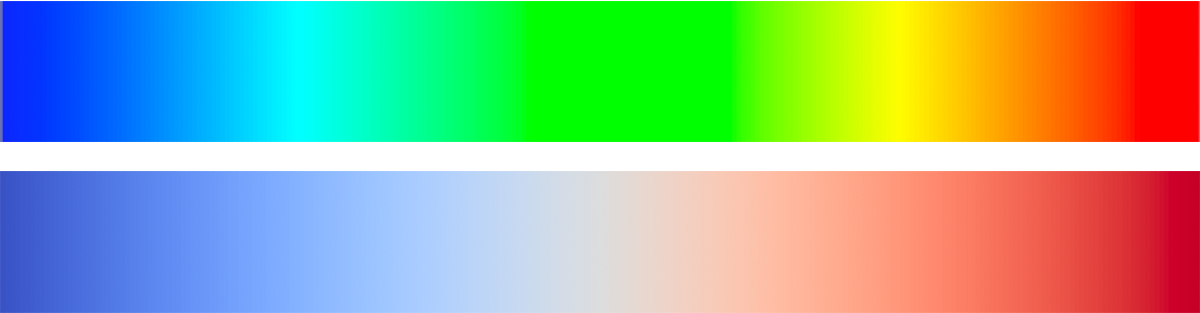
\includegraphics[width=16pc]{pics/Maps2.png}}
%\caption{The \huewheel and \coolwarm colormaps.}
%\label{r and cw}
%\end{figure}

The origins of the new default color map arise from a collaboration between climate scientists, visualization experts, and visual artists~\cite{Samsel2015}.
The team found that the existing default colors do not reveal enough detail within the high-resolution data they use.
This collaboration engendered the \blueorange colormap (Figure~\ref{fig:design:blueorange}), which better satisfies the needs of the climate scientists~\cite{Samsel2015:SC}.
This colormap is built on the same principles as the \coolwarm colormap (Figure~\ref{fig:design:coolwarm}) but with expanded ranges of contrast using more hue, saturation, and luminance.

%% Our improvement to the default ParaView colormap was an iterative process that is based on Blue Orange diverging \cite{Samsel2015:SC}, a colormap built on the same principles as the \coolwarm colormap but with expanded ranges of contrast of hue, saturation and luminance.
%% \fast, the new default in ParaView, is refined to meet the needs of the broader scientific community and adhere to the criteria above.
%% The iterations are shown in Figure \ref{4maps}.

%\subsection{The Blue--Orange Diverging}

%% \begin{figure}[h!]
%% \centerline{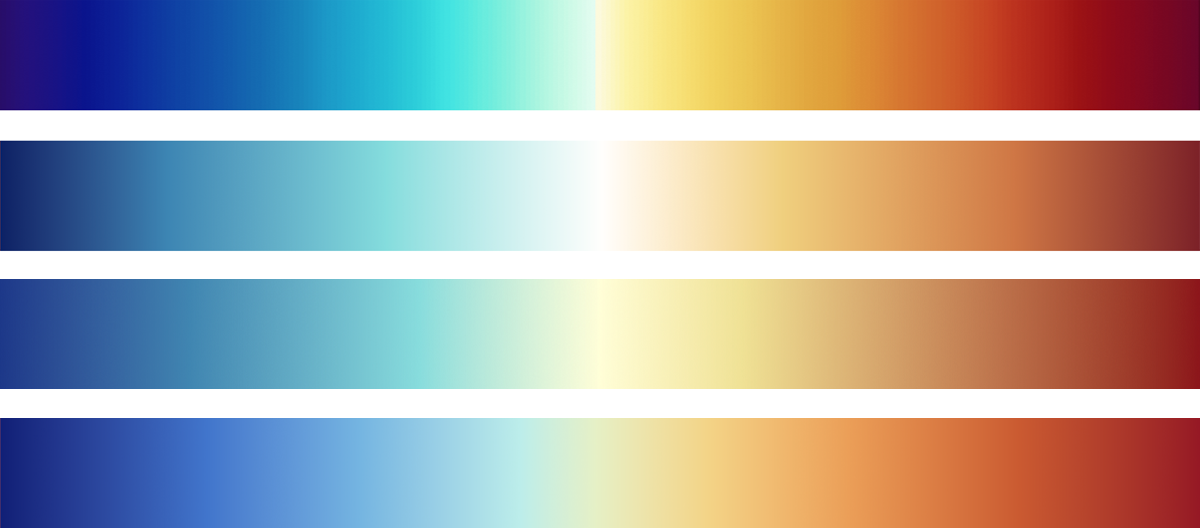
\includegraphics[width=18.5 pc]{pics/4maps.png}}
%% \caption{Top to bottom: Blue-Orange diverging colormap; first iteration - smoother center transition, lower value and saturation; increased saturation in the lower value center to assist seeing detail on white backgrounds; \fast - smoother center transition through the use of low value green hues, greater reliance on namable hues.}
%% \label{4maps}
%% \end{figure}

%% \begin{figure}[htb]
%%   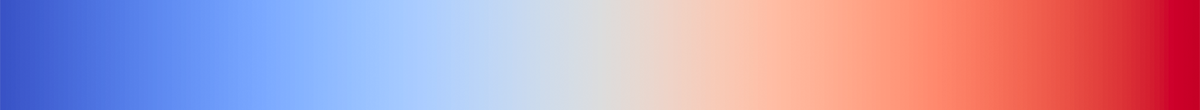
\includegraphics[width=\linewidth]{map-cool-to-warm}\\[4pt]
%%   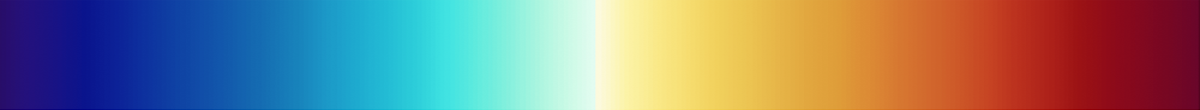
\includegraphics[width=\linewidth]{map-blue-orange-diverging}\\[4pt]
%%   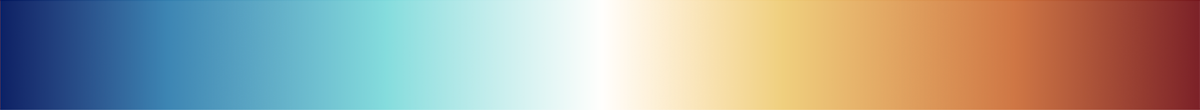
\includegraphics[width=\linewidth]{map-iteration-1}\\[4pt]
%%   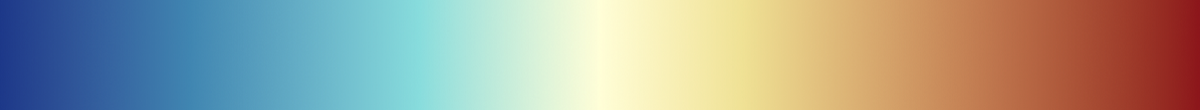
\includegraphics[width=\linewidth]{map-iteration-2}\\[4pt]
%%   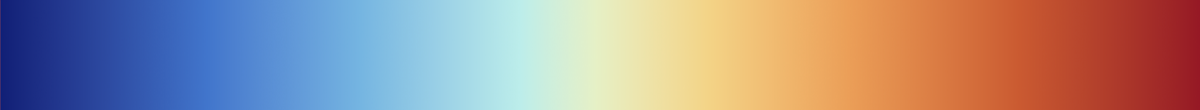
\includegraphics[width=\linewidth]{map-fast}
%% \end{figure}

\begin{figure}[htb]
  \begin{subfigure}{\linewidth}
    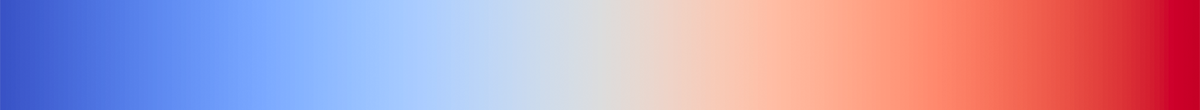
\includegraphics[width=\linewidth]{map-cool-to-warm}
    \vspace{-1.4\baselineskip}
    \caption{Original \coolwarm coolwarm.}
    \label{fig:design:coolwarm}
  \end{subfigure}\\[4pt]
  \begin{subfigure}{\linewidth}
    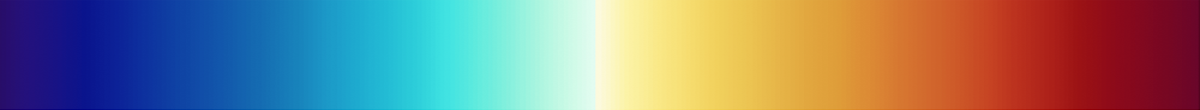
\includegraphics[width=\linewidth]{map-blue-orange-diverging}
    \vspace{-1.4\baselineskip}
    \caption{\blueorange colormap.}
    \label{fig:design:blueorange}
  \end{subfigure}\\[4pt]
  % The map iterations are now covered in Figure \ref{fig:iteration}. These iterations are no longer references and are a bit confusing now, so I'm removing them.
  %\begin{subfigure}{\linewidth}
  %  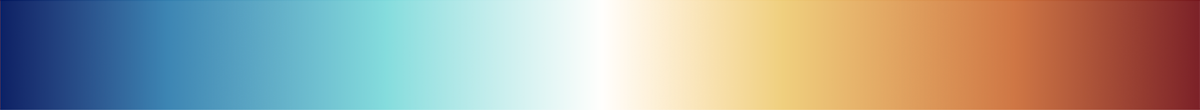
\includegraphics[width=\linewidth]{map-iteration-1}
  %  \vspace{-1.4\baselineskip}
  %  \caption{Iteration 1: Smooth center, brighter, less saturated.}
  %  \label{fig:design:iteration1}
  %\end{subfigure}\\[4pt]
  %\begin{subfigure}{\linewidth}
  %  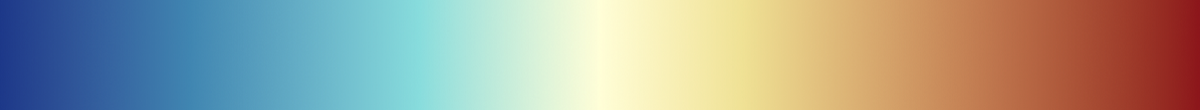
\includegraphics[width=\linewidth]{map-iteration-2}
  %  \vspace{-1.4\baselineskip}
  %  \caption{Iteration 2: Yellow hue in the center.}
  %  \label{fig:design:iteration2}
  %\end{subfigure}\\[4pt]
  \begin{subfigure}{\linewidth}
    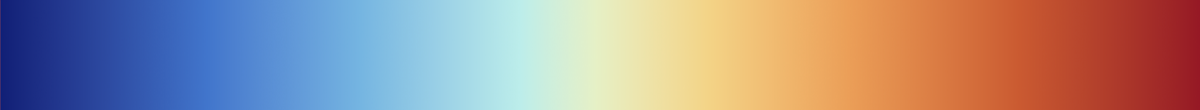
\includegraphics[width=\linewidth]{map-fast}
    \vspace{-1.4\baselineskip}
    %\caption{\fast: More smoothing and increase in nameable hues.}
    \caption{Final \fast colormap.}
    \label{fig:design:fast}
  \end{subfigure}
  \caption{
    Transition of the default ParaView color map from the original (top) to final (bottom) designs.
  }
  \label{fig:designs}
\end{figure}

The \blueorange colormap improves on the discriminating power of \coolwarm by increasing the range of all available color channels without violating robustness to colorblindness.
First, the brightness range is expanded by dropping the brightness at each end.
This increases the luminance profile, which is known to be the most powerful channel for visual discrimination, particularly for high-frequency data \cite{Ware2019}.
The hue range is also expanded by mixing green into the lighter colors and moving the darker colors toward purple.
The saturation is also significantly increased across the color map to bring more vibrancy and more clearly distinguish between the hues.
User studies like that in Figure~\ref{Ware}
show the \blueorange colormap to be better than the original \coolwarm colormap and overall one of the best performing colormaps \cite{Ware2017,Ware2019,Turton2017}.

\begin{figure}
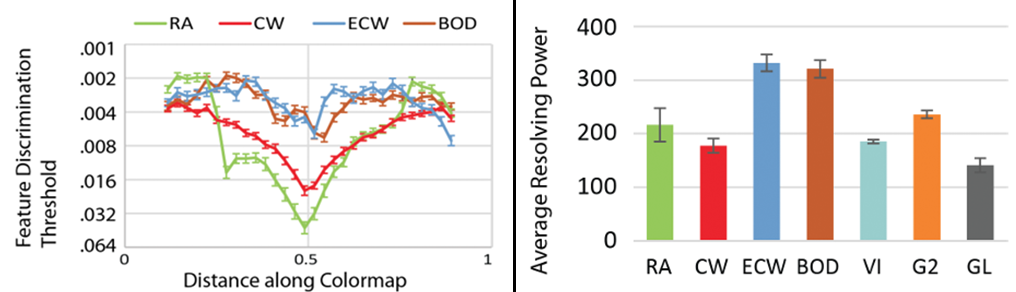
\includegraphics[width=\linewidth]{pics/Ware17.png}
\caption{This chart by Ware et al \cite{Ware2019} documents the significant increase in discriminatory power of \blueorange. \colormap{Extended Cool-Warm} also shows increased discriminatory power, which it achieves by spanning an even wider range of luminance. However, this exacerbates the shading issue illustrated in Figure~\ref{fig:3d-shading}.}
\label{Ware}
\end{figure}

The success of the \blueorange colormap, which shares features with \coolwarm, suggests that improvements could be made.
A reasonable impulse would be to simply establish \blueorange as the default ParaView colormap.
However, the \blueorange colormap design comes from a particular collaboration with climate scientists studying ocean temperature and is thus developed specifically for their needs.
Because it was created with a narrow focus of customers, it has some characteristics that make it unsuitable for more general application.

%\begin{figure*}[htb]
%  \centering
%  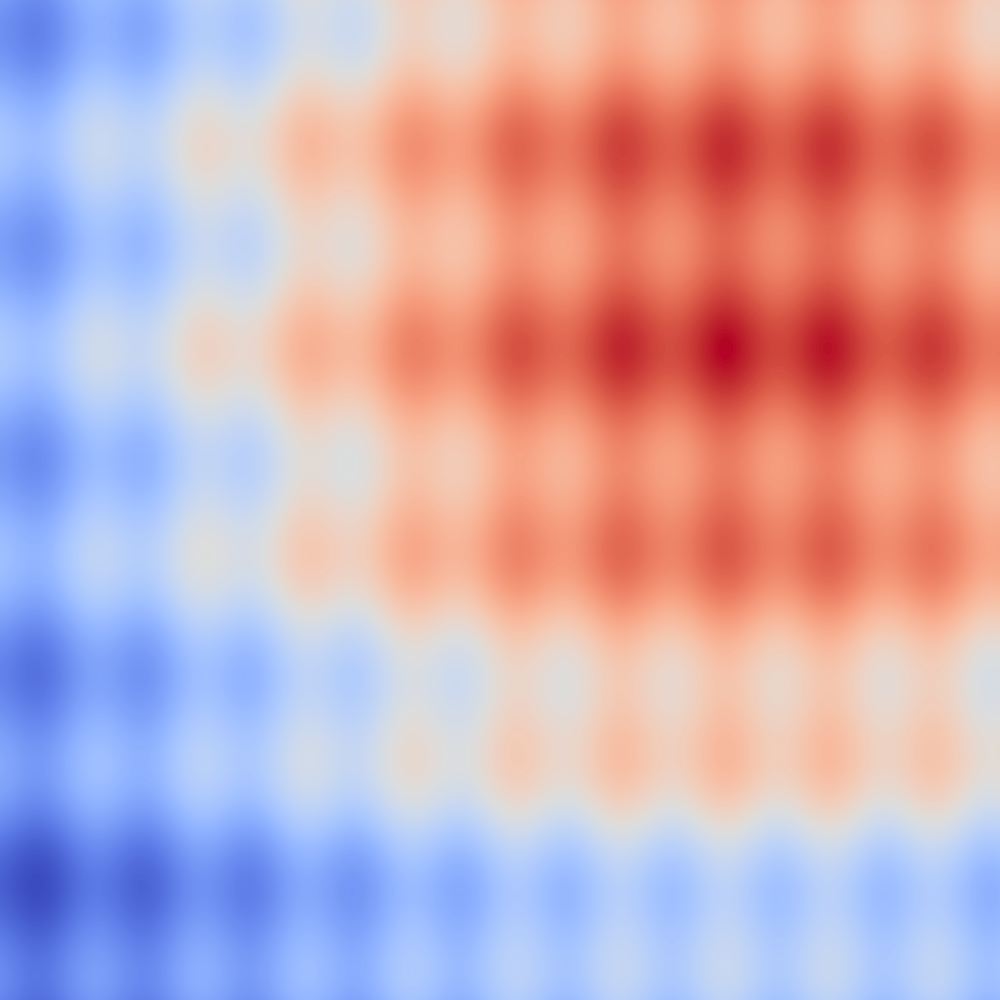
\includegraphics[width=.32\textwidth]{smoothness-cool-warm}
%  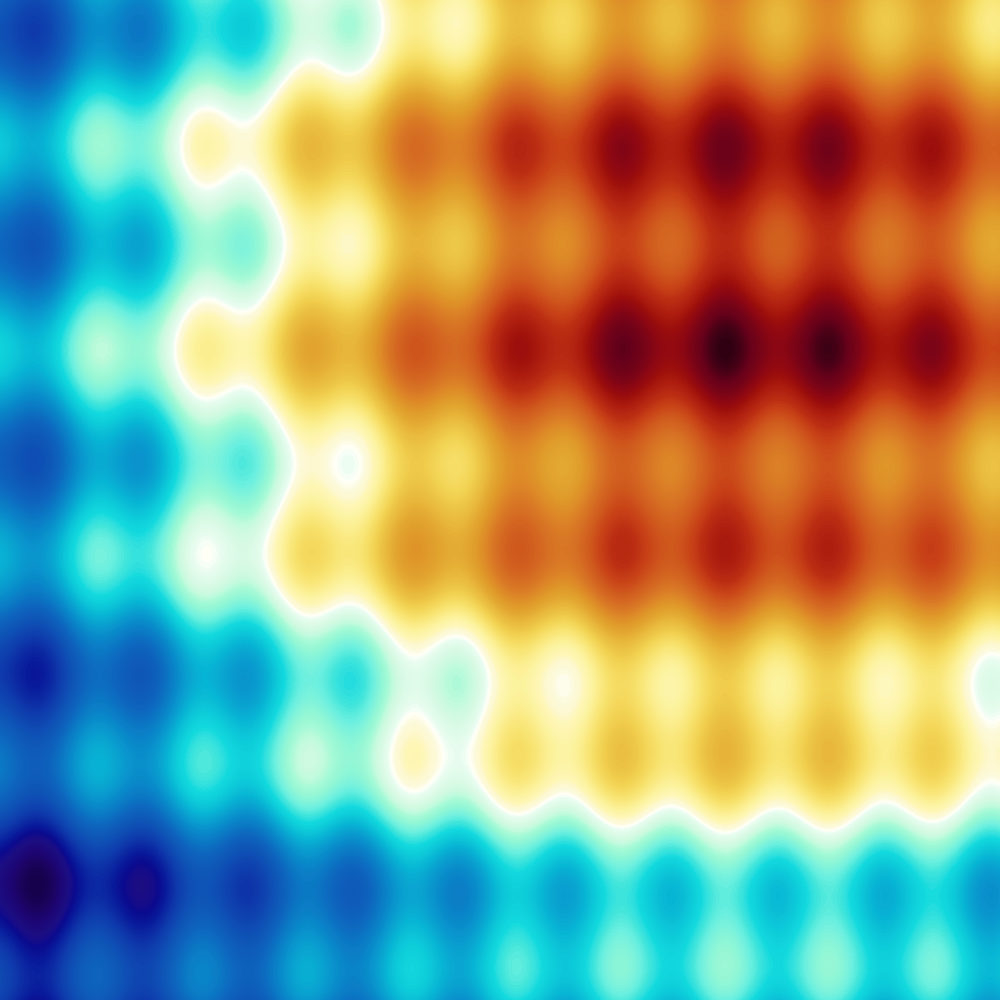
\includegraphics[width=.32\textwidth]{smoothness-blue-orange}
 % 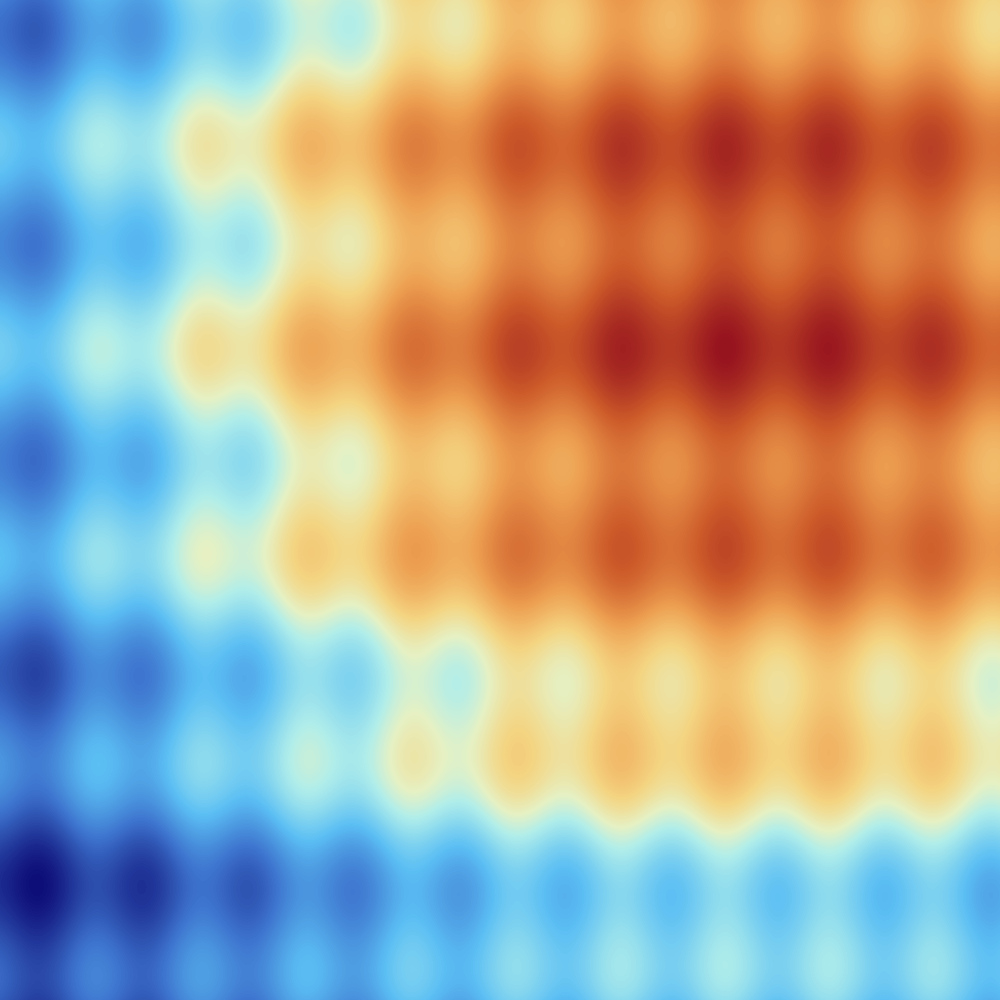
\includegraphics[width=.32\textwidth]{smoothness-fast}
%  \caption{
%    Demonstration of the smoothness of colormaps.
%    The \coolwarm colormap (left) is smooth throughout.
%    The \blueorange colormap (middle) has a sharp ``peak'' at the center white point where the luminance transitions from increasing to decreasing.
%    Our final \fast colormap (right) smooths out this middle point.
 % }
%  \label{fig:smoothness}
%\end{figure*}

\begin{figure*}[htb]
\centering
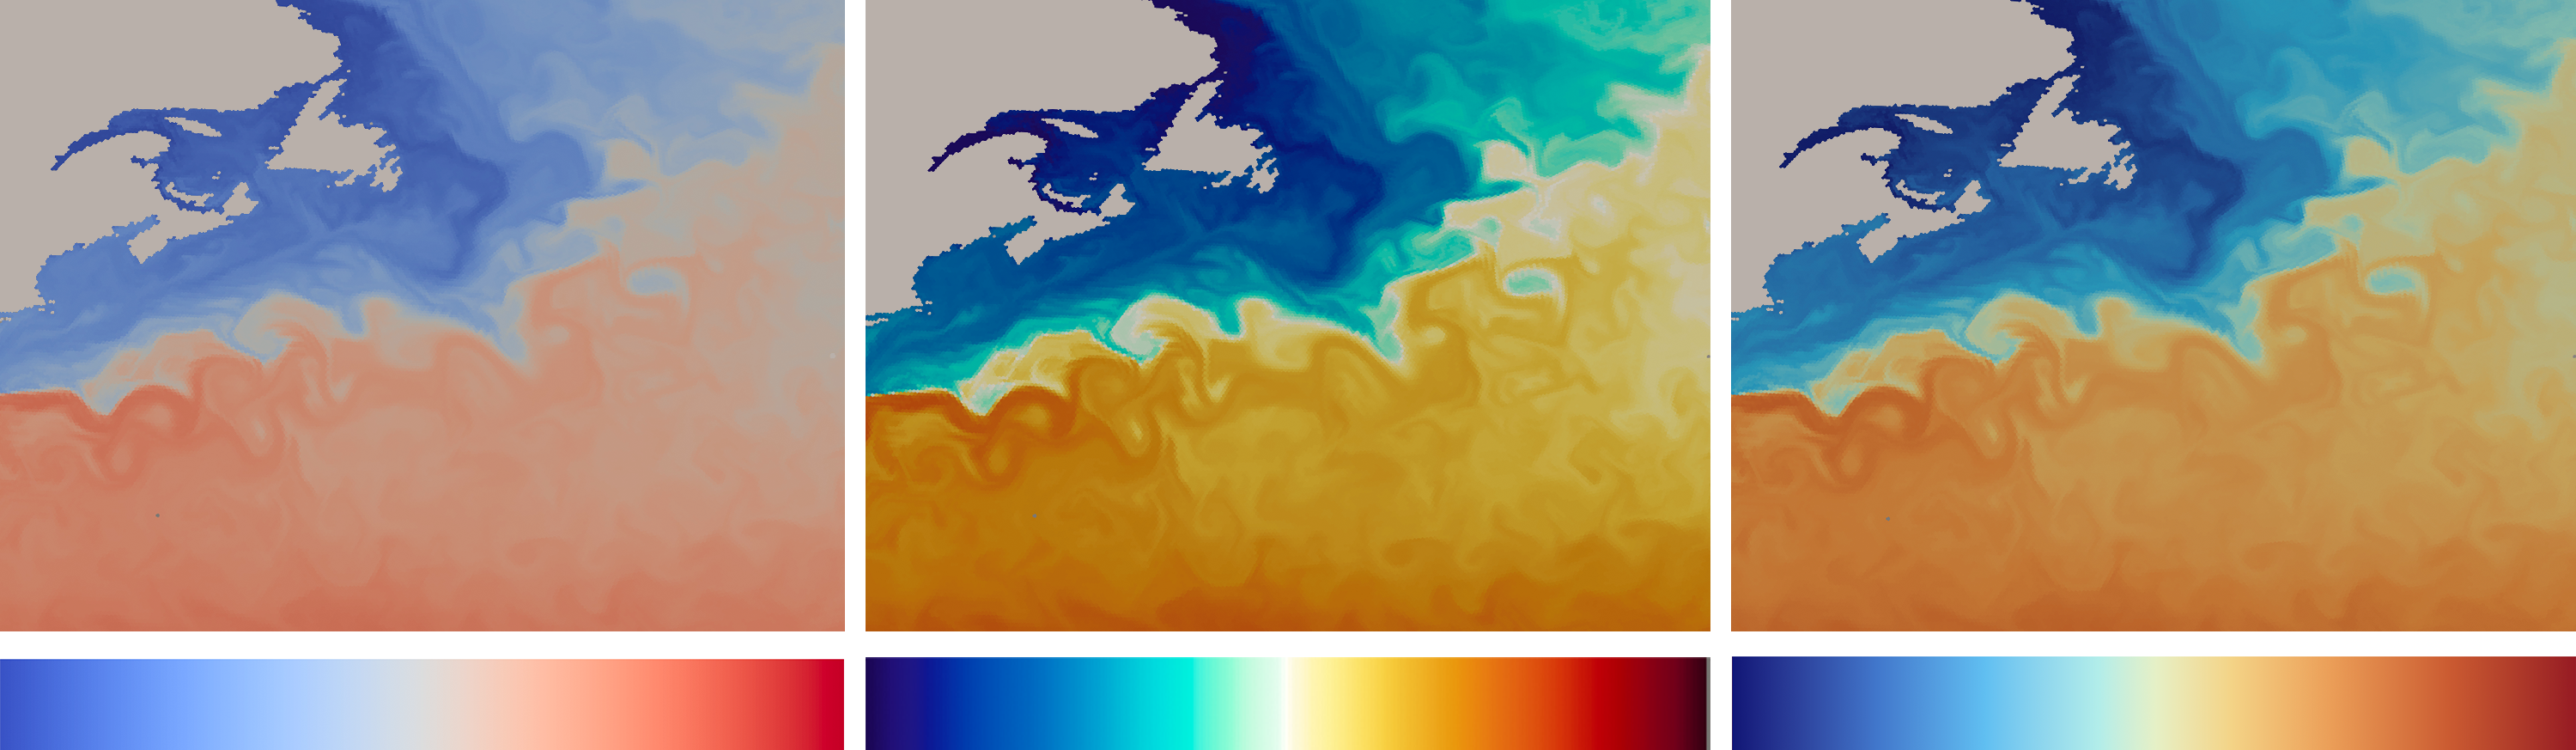
\includegraphics[width=\textwidth]{pics/Ocean2.png}
\caption{Demonstration of the smoothness of colormaps using E3SM ocean temperature data.
    The \coolwarm colormap (left) is smooth throughout.
    The \blueorange colormap (middle) has a sharp ``peak'' at the center white point where the luminance transitions from increasing to decreasing.
    Our final \fast colormap (right) smooths out this middle point. }
\label{fig:smoothness}
\end{figure*}


\begin{figure}[htb]
 % \centering
  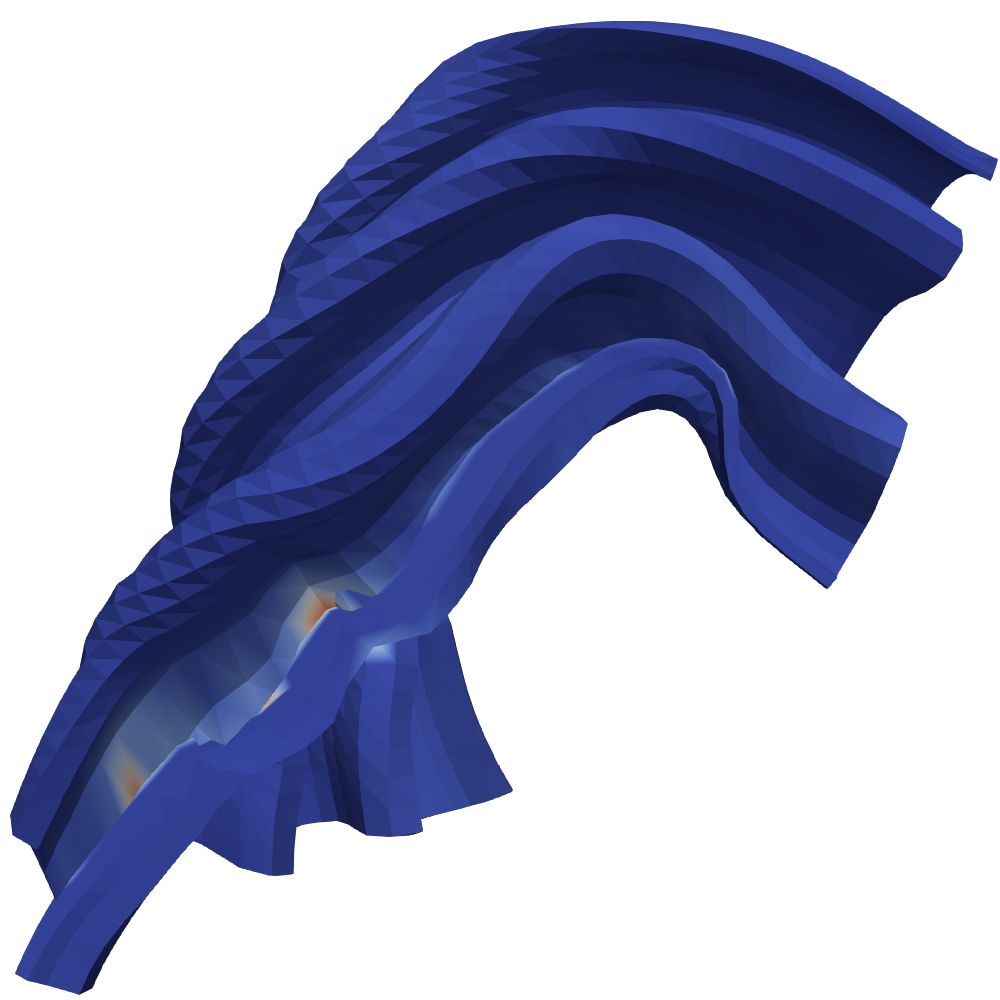
\includegraphics[width=.15\textwidth]{shading-cool-warm}
  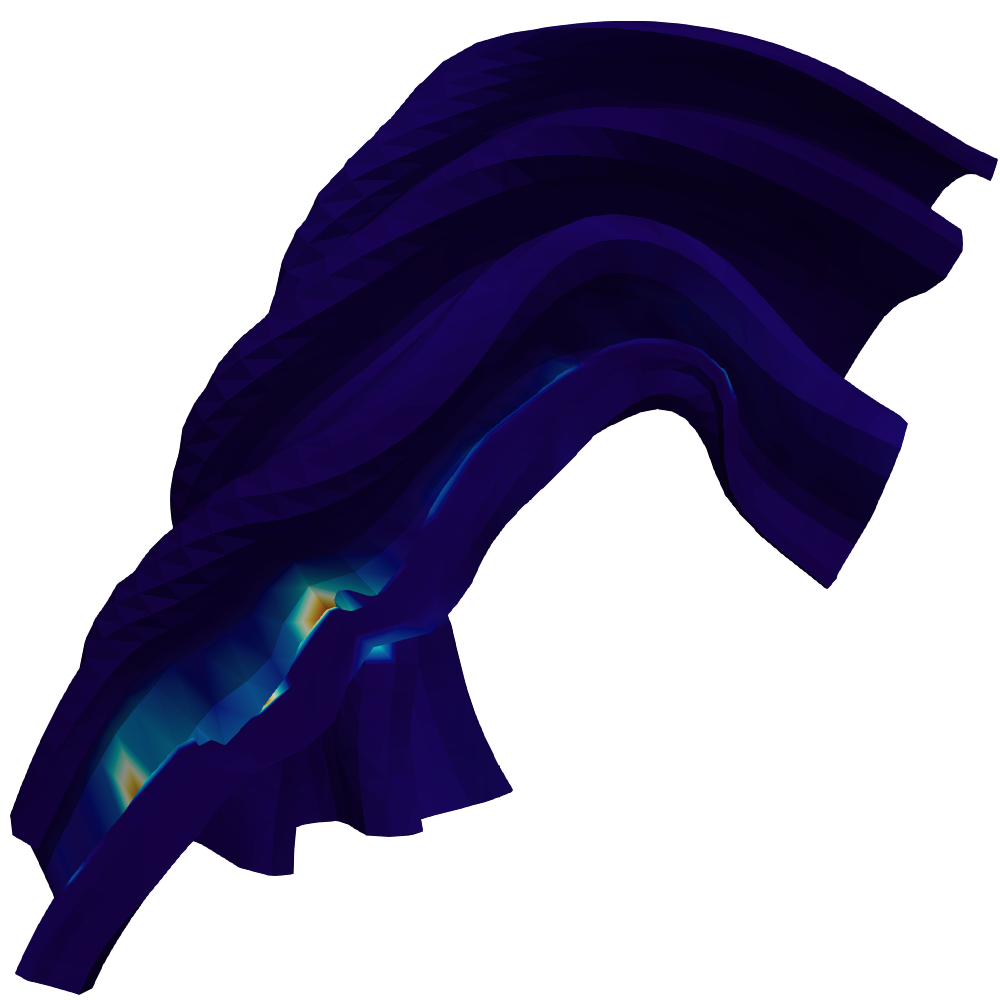
\includegraphics[width=.15\textwidth]{shading-blue-orange}
  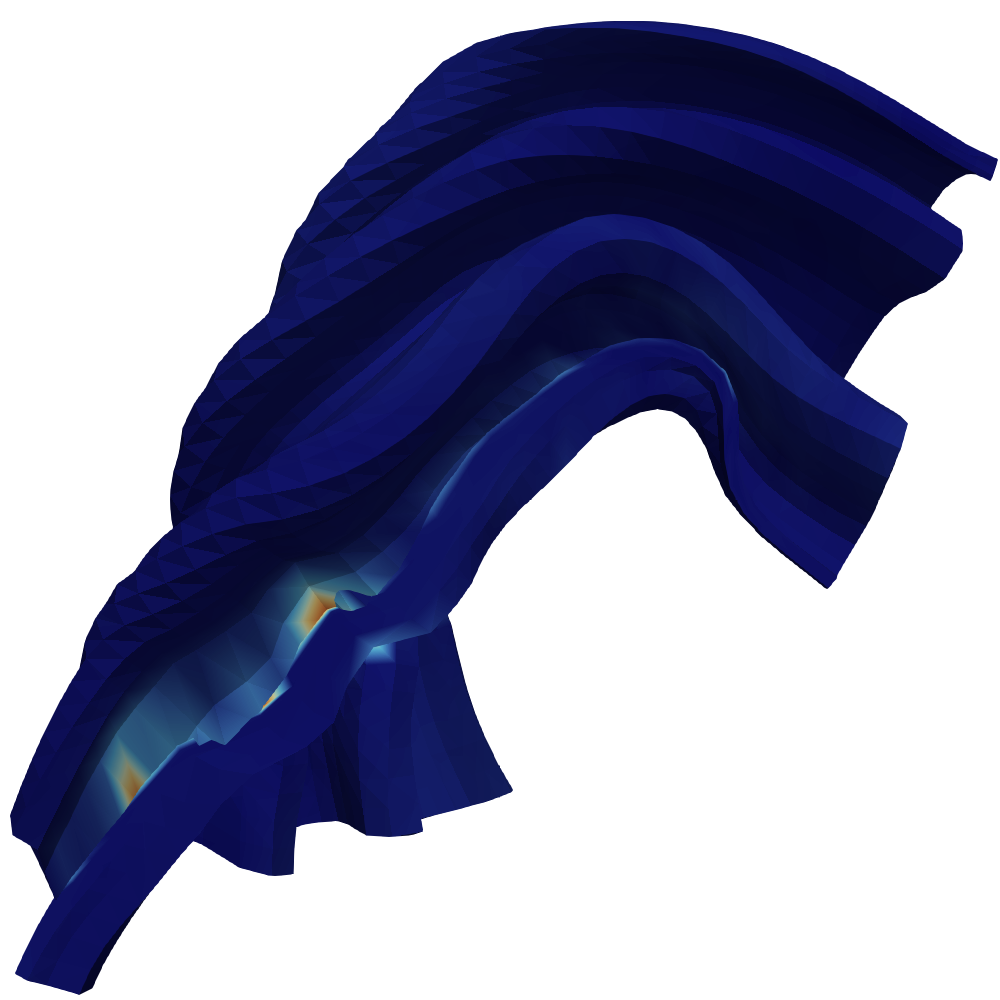
\includegraphics[width=.15\textwidth]{shading-fast}
  \caption{
    Effect of colormap darkness on shading.
    The colors at the ``dark'' ends of the \coolwarm colormap (left) are kept bright enough to easily discern shading.
    The \blueorange colormap (middle) becomes too dark perceive shape.
    Our final \fast colormap (right) is as dark as we could make it (for a better luminance range) while still making shapes detectable.}
  \label{fig:3d-shading}
\end{figure}

First, there is a strong focal point in the center where the map brightness peaks at white.
This peak creates a distinct line across the surface as can be seen in Figure~\ref{fig:smoothness}.
This may be desirable for data where the middle of the range has a value of specific importance, but it is imperfect for general data and violates the smoothness characteristic we desire.
To correct for this, we smooth the transition of brightness and saturation through the center.
That said, we do not make this transition perfectly smooth as doing so would drop the discriminability in this section.
We see this as one of the problems with discriminability in the \coolwarm colormap, so we compromise on a mostly smooth transition.

Second, the dark ends of the \blueorange colormap can interfere with 3D shading as shown in Figure~\ref{fig:3d-shading}.
%\fix{Ken, The best way to illustrate this is to build on the crushed can vis. I am happy to make the figure if you want to forward the state file you use or we can leave this out. } However that can be mitigated using lighting as shown in Figure \ref{wind3}.
This is of little concern for the original customers who do not deal with complex shapes, but it is quite important for our general purpose map.
This problem is corrected by trimming, brightening, and raising the saturation of the dark ends of the map.
Again, we are making a compromise leaning more toward discriminability, making the shading just visible in the worst case of coloring everything by the darkest color.

%\begin{figure*}
%\centerline{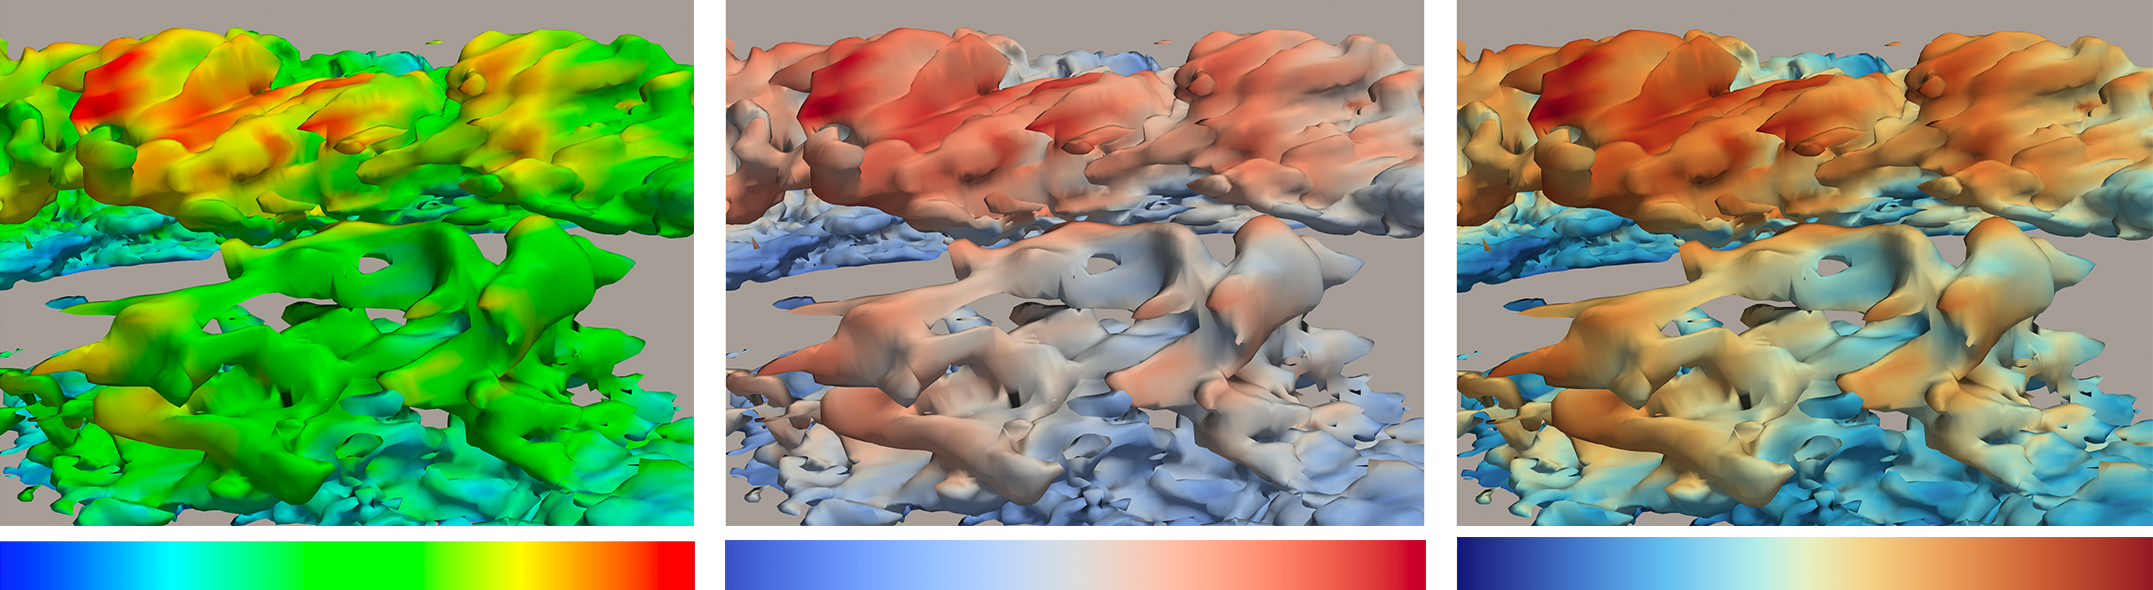
\includegraphics[width=\textwidth]{3VolumeHistory2}}
%\caption{
 % Surface data colored using the \huewheel colormap (left), \coolwarm colormap (middle), and \fast (right) \fix{The idea here was to show the maps on a complex 3D surface. }.
%}
%\label{wind3}
%\end{figure*}
Based on these needed adjustments to the \blueorange colormap, we constructed many candidate maps.
A sample of these maps is shown in Figure~\ref{fig:iterations}, documenting the changes and illustrating 
the impact. These maps were evaluated using $\Delta$E discriminability metric in CCC Tool \cite{Nardini2021}.
% I am removing the sentence below because I do not understand it. The reference is to Figure 2c, but the text seems to describe Figure 5. But if that is the case, it seems like it is just reiterating the previous sentence, in which case we can just remove it.
%Figure~\ref{fig:design:iteration1} illustrates the evolution of \blueorange, left to \fast, right.

Starting on the left, in column A, one can see that \blueorange produces saturated, detailed renderings with a clear delineation between the cool and warm sections.
The first goal was to lower the center focal point and equalize the uniformity of the steps within the colormap, which was achieved in the modified colormap in column B.

In column C, we sought to further smooth the center range as well as experiment with lightening the end values to address the shading concerns shown in Figure~\ref{fig:3d-shading}.
We also added a yellow tint to the center values to prevent bright colors from blending into white backgrounds as shown in Figure~\ref{fig:middle-point}.

\begin{figure}[tb]
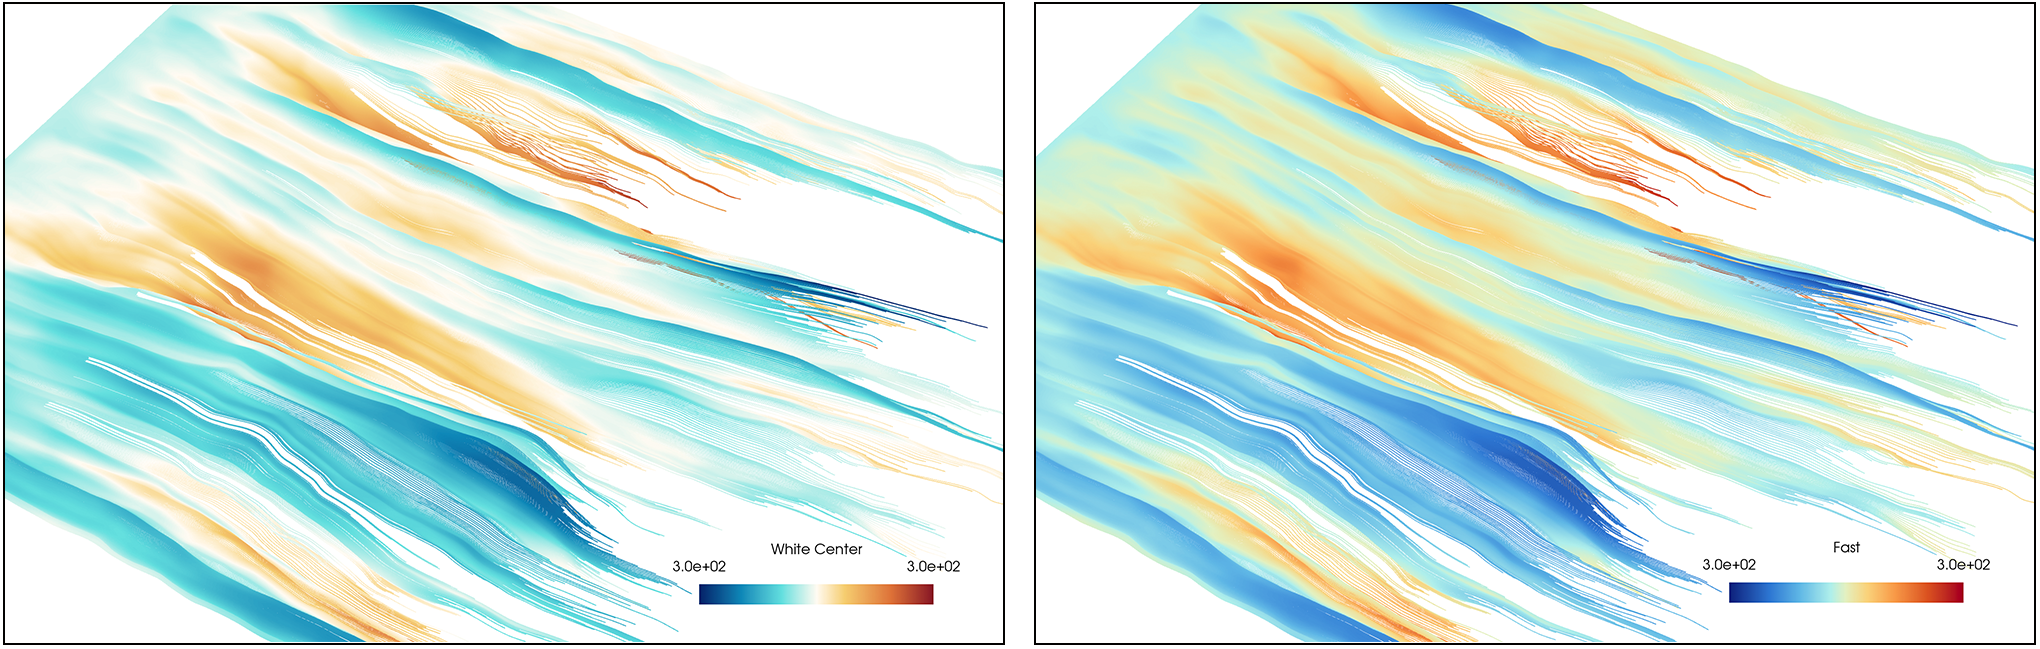
\includegraphics[width=\linewidth]{Final_Pics/white_yellow.png}
\caption{Wind streamlines using our first iteration of \fast containing a white center value and the final version of \fast with saturation increased in the mid-range.}
\label{fig:middle-point}
\end{figure}

\begin{figure*}[htb]
  \centering
  \includegraphics[width=\textwidth]{Final_Pics/Iterative5letters.png}
  \caption{
    Iterative design from the \blueorange colormap (A) to our final design of \fast (E).
    The impact of each iteration is demonstrated on three types of data: 2D continuous combustion data (LLNL), streamlines of wind from a fire simulation (LANL), and volumetric data of smoke from the same fire simulation.
    %\fix{The prose refers to columns labeled A--E, but no such labels are in the figure. --Ken}
  }
\label{fig:iterations}
\end{figure*}



However, the discriminatory power of this colormap was significantly compromised from these previous changes.
In response, we increased the saturation across the colormap and extended the warm hues toward purple for the iteration in column D.
This map was close but our evaluation methods showed lower discriminability in the center ranges. 


To compensate, we increased the saturation again and shifted the turquoise region toward the center to provide extra discrimination in this region, resulting in the final \fast colormap shown in column E.
This subtle increase in detail is visible in the 2D data of Figure~\ref{fig:iterations} while still maintaining a good middle point and 3D shading behavior.




%\fix{I removed a reference to Figure~\ref{fig:designs}, suggesting that those were the maps with candidates. As I recall, the refinement was pertubations of Figure~\ref{fig:design:iteration2} only. We used to have a figure for that. It got removed, but that's probably OK. (Ken)}
These candidate colormaps manifest different balances of our criteria: the luminance range to balance discriminability and 3D shading, different luminance adjustments at the centerpoint to balance uniformity and smoothness, different hue ranges to balance discriminability and order. 

%Figure \ref{fig:iterations} illustrates the process of balancing maximum discriminatory power, uniformity and smoothness while maintaining robustness to 3D shading and colorblindness. Specifically, the changes made from left to right are: our starting point, blue-orange divergent; aiming for smooth uniform transitions across the colormap; further smoothing of the center range; increasing the discriminatory power by expanding both the value and saturation range across the colormap; maintaining the discriminatiory power at in the middle range as well as unifying and smoothing the transitions by shifting the hue distributions.

Figure \ref{fig:iterations} illustrates the applications of these candidate colormaps to three types of data - continuous 2D data, streamlines, and volumetric data.



%Some colormaps performed slightly better on specific types of data: streamlines; volumes; 2D surfaces and point data.
%The differences aligned with the density of the data and the background color.
%Using this information, the team balanced the considerations between the types of data, user preferences and characteristics of the colormaps.

%Once the colors of the map were agreed on, we made final adjustments for smoothness, uniformity, and discriminatory power.
Finally, a sequence of control points was chosen for a piecewise-linear interpolation of colors in CIELAB space with a preference to minimize their number.
In practice, users sometimes wish to modify a colormap to their purpose.
For example, users may wish to adjust the colors to highlight particular regions of their scalar data.
This cannot be done easily with larger numbers of control points, so we removed any control points where interpolation produces nearly identical results.
Our final design has nine control points as it is the minimum needed to produce a smoothly transitioning map that moves through the hues we have selected.


%% \begin{figure}
%% \centerline{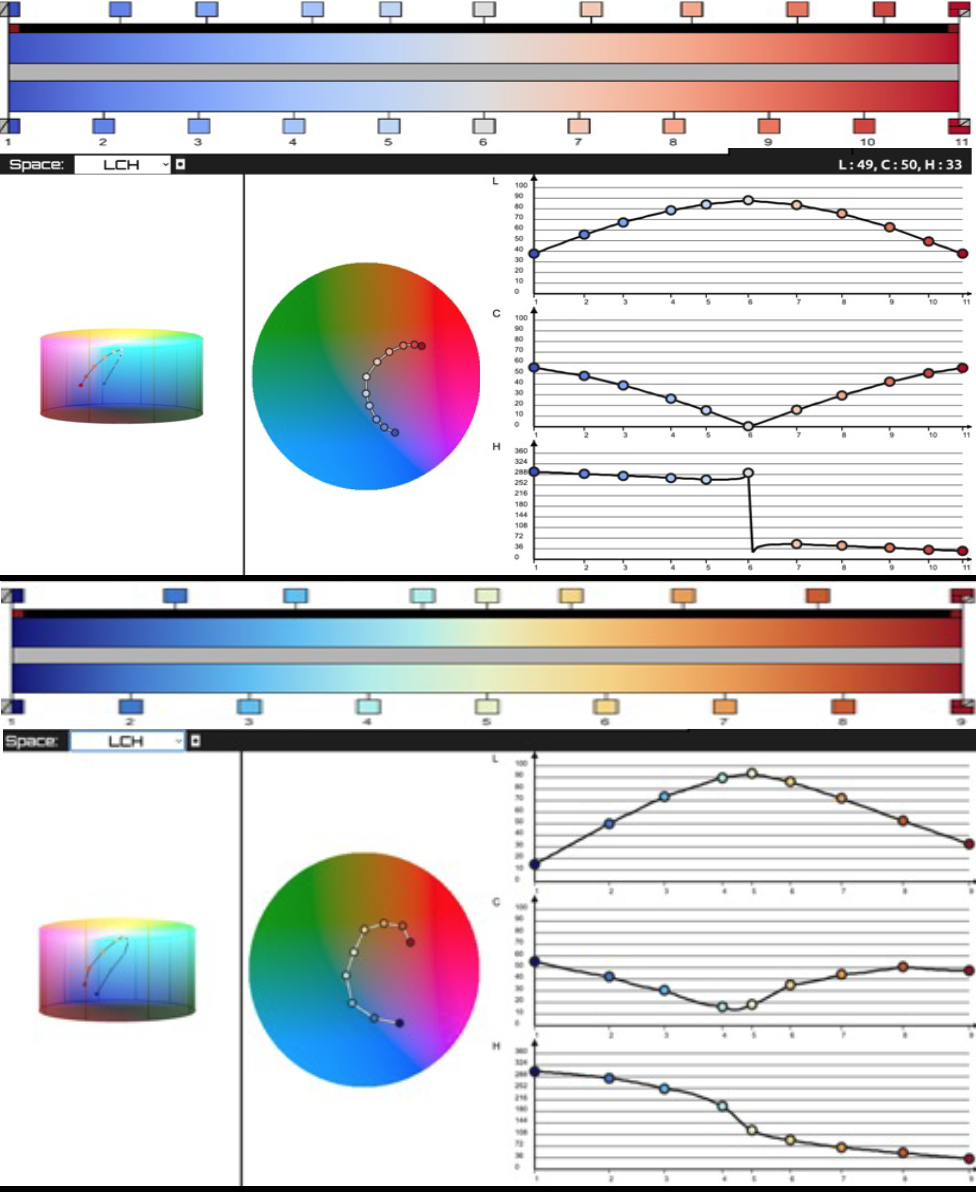
\includegraphics[width=18.5 pc]{pics/Charts.png}}
%% \caption{Colormap properties displayed in CCC Tool \cite{Nardini2021} for \coolwarm and \fast.}
%% \label{Charts}
%% \end{figure}




\section{USER FEEDBACK}

% Commenting out these two paragraphs. They cover the same ground as the last two paragraphs of the previous section, and neither has anything to do with user feedback.

%% This initial set of colormaps spawned a discussion among the ParaView development team and produced some mild opinions. These were used to cull down to three sets of maps that varied by: the luminance level, (darkness), at the ends of the colormap; the saturation levels across the colormap; and the smoothness and value of the center transition from cool to warm. All these colormap variations considered retained their perceptual uniformity and robustness to colorblindness.

%% Once the colors of the map were agreed on, the team optimized the colors for smoothness and adjusted colors for equal distribution of discriminatory power.
%% We decided on nine control points as it was the minimum needed to produce a smoothly transitioning map that moves through hues.
%% See Figure \ref{Charts}.
%% In practice, users sometimes wish to modify a colormap to their purpose.
%% For example, users may wish to adjust the colors to highlight particular regions of their scalar data.
%% This cannot be done easily with larger numbers of control points, so we removed any control points where interpolation in CIELAB space produced similar results.

As we neared completion of the new colormap design, the development team wanted feedback from current users about these changes before being affected by them.
Sandia National Laboratories has a strong ParaView user base and an active support team for them.
The ParaView support team sent an email to the Sandia ParaView users informing them of planned changes and welcoming any feedback.

Of the roughly 800 users receiving the email, 18 responded back with comments about the change of the default colormap from Cool to Warm to Fast.
Of these, 15 expressed a clear preference for the new colormap.
Only 1 preferred the original Cool to Warm colormap with the remaining 2 expressing no preference of one over the other.
Although no formal study has been done, we see this as a clear general preference to the new colormap.

\begin{figure*}[htb]
  \centering
  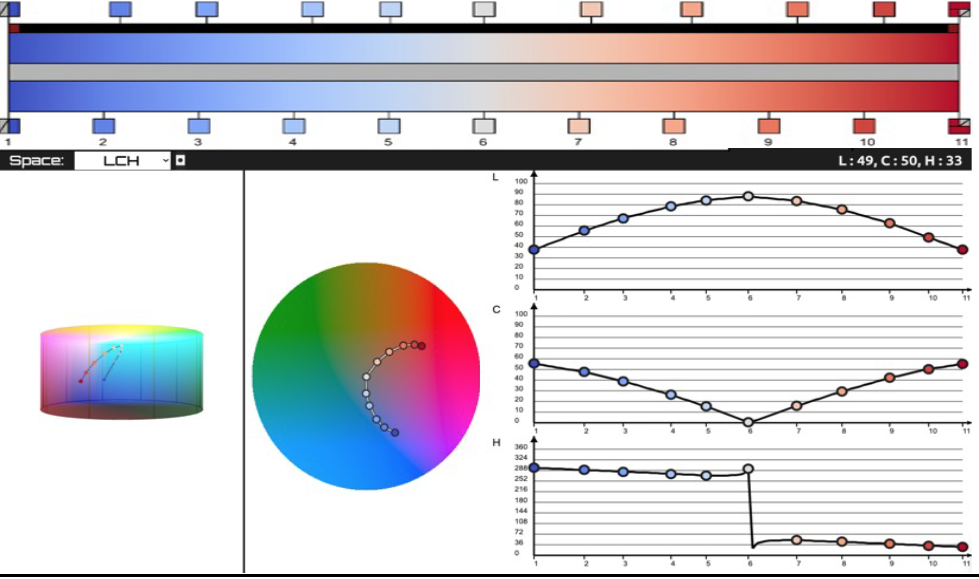
\includegraphics[width=.49\textwidth]{Final_Pics/chart_CW.png}
  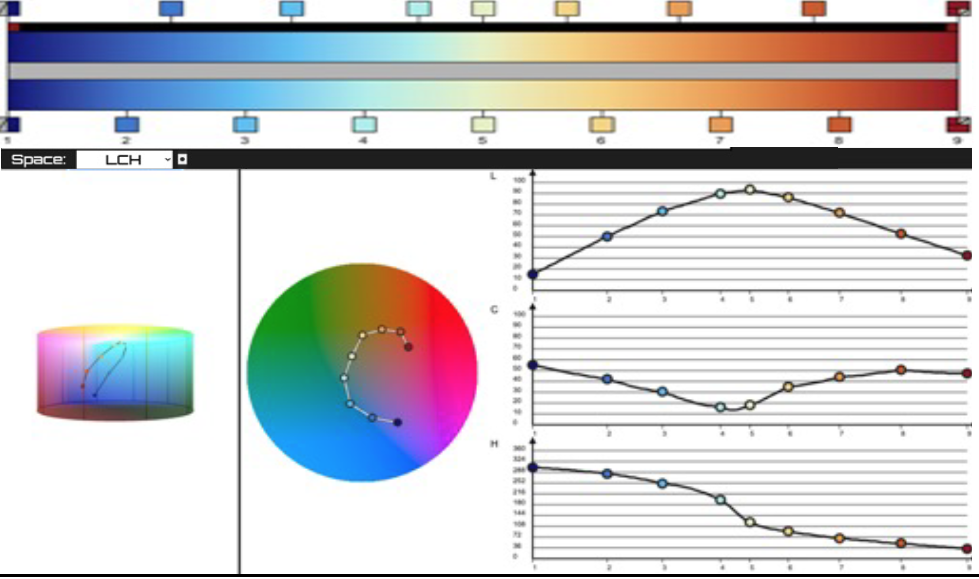
\includegraphics[width=.49\textwidth]{Final_Pics/chart_Fast.png}
  \caption{Colormap properties displayed in CCC Tool \cite{Nardini2021} for \coolwarm (left) and \fast (right).}
  \label{Charts}
\end{figure*}


\section{PERCEPTUAL EVALUATION}

Although we have not yet had a chance to perform formal human subject studies, we are confident that \fast will outperform its predecessor, \coolwarm, in terms of discriminability.
In particular, \fast has a higher $\Delta$E discriminability metric.
As measured by CCC Tool~\cite{Nardini2021}, \coolwarm has an average local CIE$\Delta$E2000 discriminability score of 120 whereas \fast has a score of 174, and the other discriminability metrics similarly show improvements with \fast.
All that said, we recognize that \fast%
%, shown in Figure \ref{Ast},
likely performs less well in general than the \blueorange colormap it is based on.
This is out of necessity to adjust for the smoothness and robustness to shading on 3D surfaces.

The \coolwarm colormap was designed about 15 years ago to move away from the \huewheel colormap and its rainbow colors because of the strong evidence at the time of its poor perceptual properties~\cite{Rogowitz1998,Borland2007,Ware1988,Light2004}.
In the interim, multiple colormaps based on the hues of the rainbow that correct some of the problems of the \huewheel have been designed.
More recent research suggests that added hues and more nameable colors can assist in color differentiations that are not otherwise explained by our perceptual color models \cite{Reda2021}.
This leads some to suggest that perceptually correct colormaps based on rainbow colormaps might be favorable \cite{Ware2023}.
Although the \fast colormap does not incorporate all rainbow hues, it does improve dramatically over the hues provided by \coolwarm as seen in the hue plots of Figure~\ref{Charts}.

\fast also has more namable colors than its \coolwarm predecessor.
Using the color categorization tendency metric proposed by Reda \cite{Reda2022}, \fast once again exceeds \coolwarm.
Using a color name similarity threshold of 0.6 (as was used by Reda), \coolwarm has a categorization tendency metric of 310 whereas \fast scores 369.
That said, \fast could likely be improved further by completing the rainbow with distinctive green hues (much like the \turbo colormap~\cite{Mikhailov2019} does).
However, these are all recent observations deserving more study, particularly for effects beyond discriminability.
Thus, we are not ready to loop back around to the full hues of a rainbow.


\section{CONCLUSION}

Our final iteration of the new colormap, which we dub ``\fast,'' is demonstrated in Figure~\ref{Ast} as well as numerous other figures in this paper.
This colormap is provided as one of the available colormaps in ParaView~5.12 and will become the default colormap in ParaView~5.13.

Revisiting the criteria presented at the beginning of this paper, we feel there is a clear advantage of the new colormap.


\begin{figure}
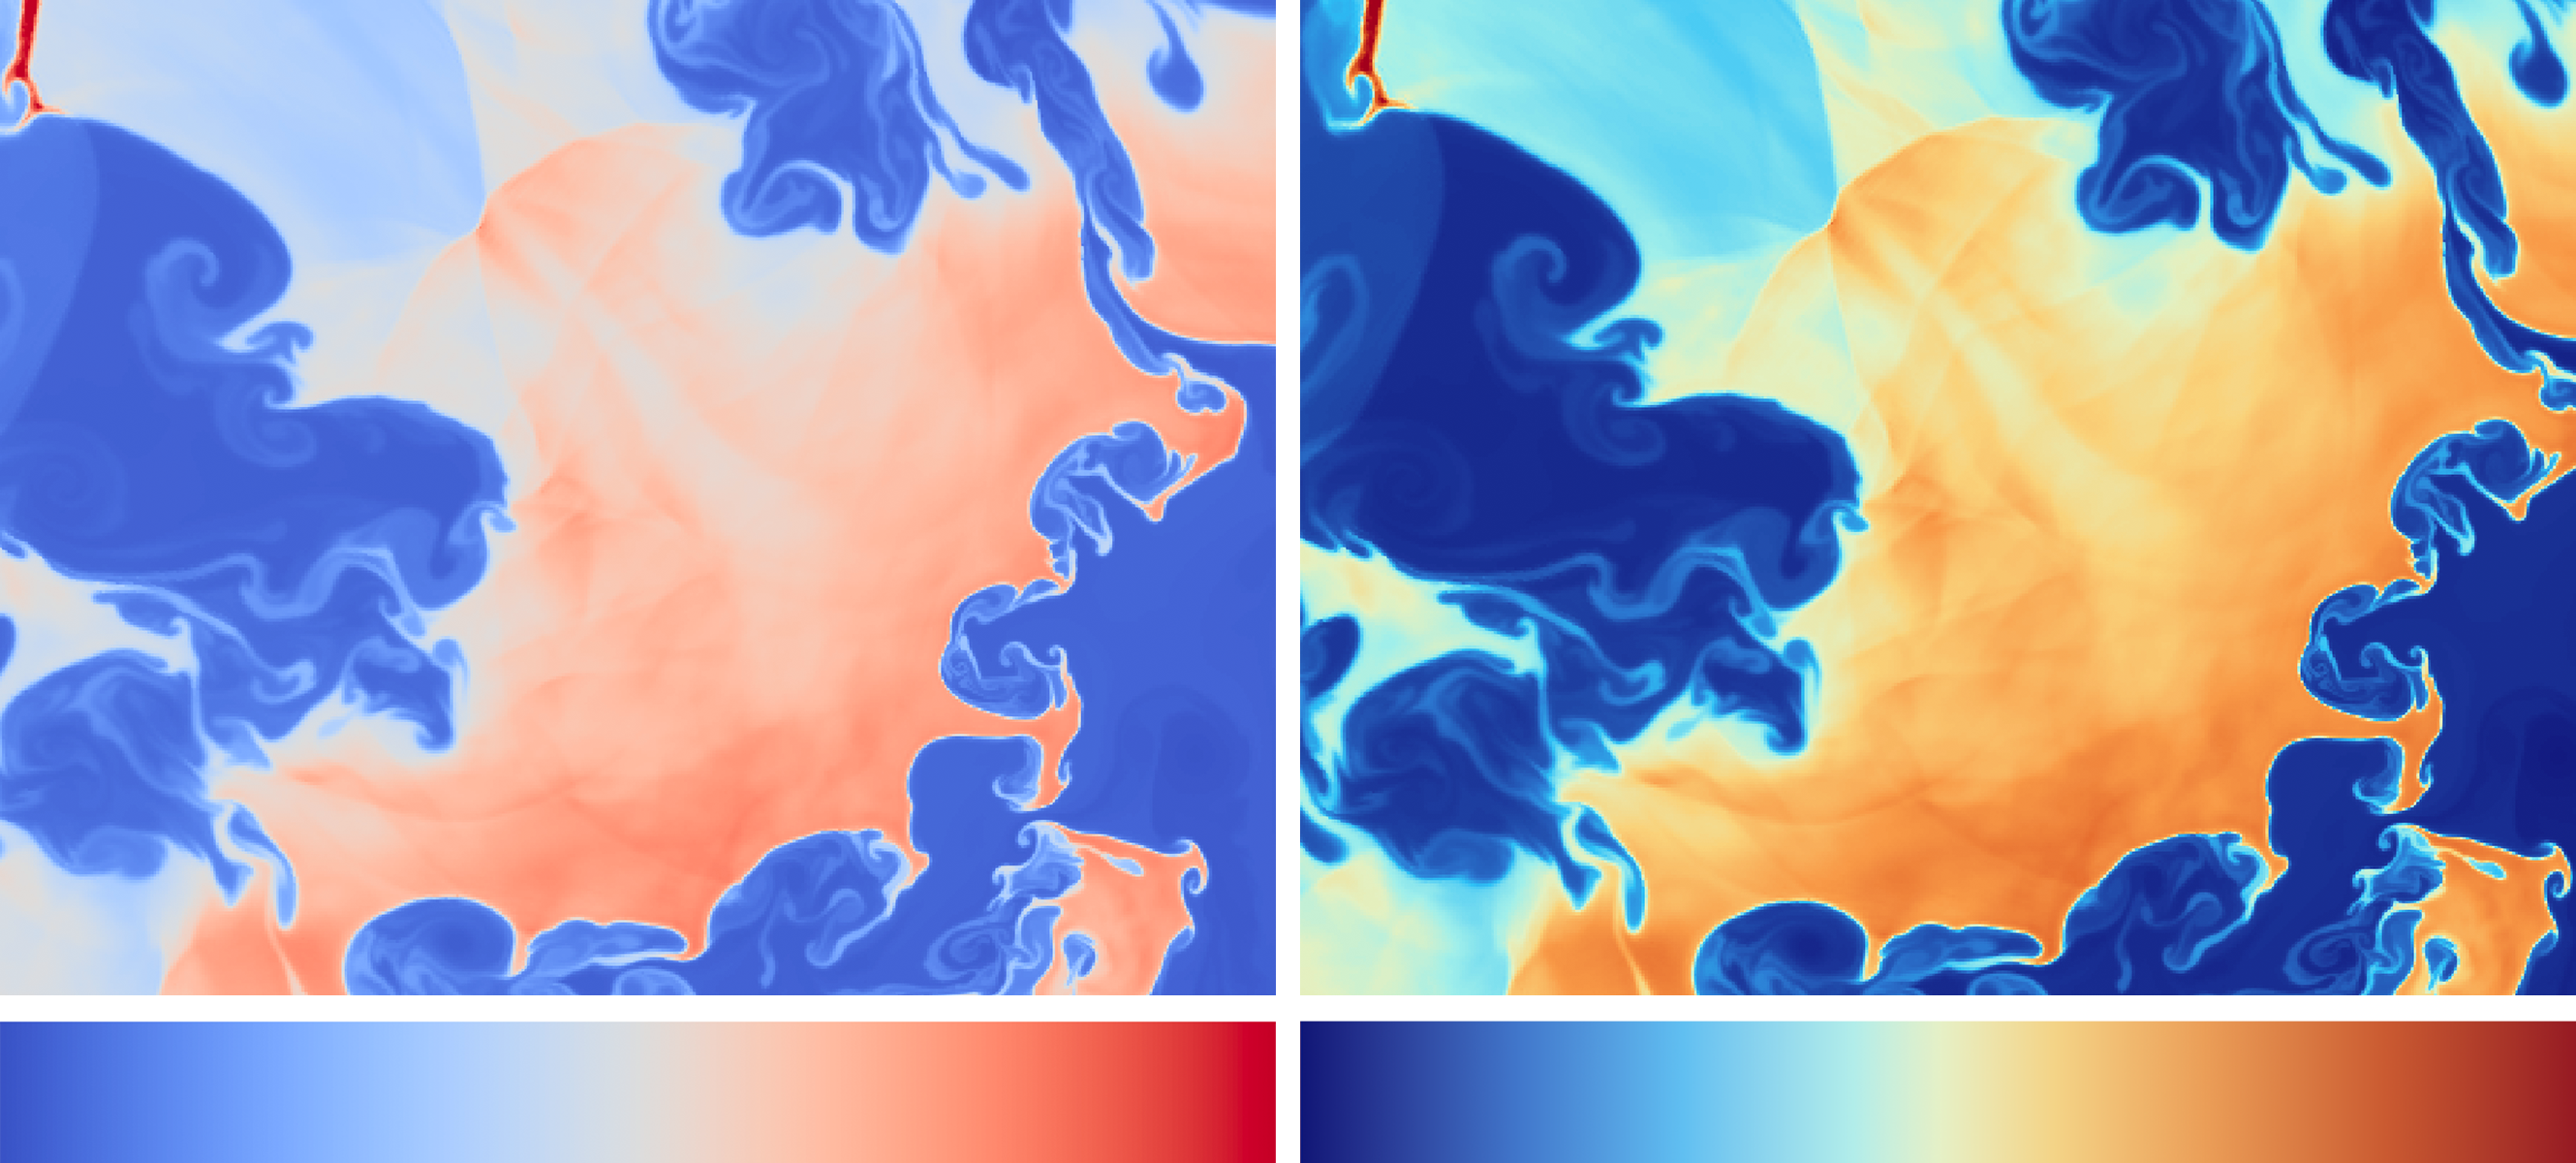
\includegraphics[width=\linewidth]{pics/Larsen2.png}
\caption{Combustion simulation (Larsen, LLNL) of \coolwarm (left) and \fast (right) colormaps demonstrating to discriminatory power in the mid-range of data values.}
\label{Larsen}
\end{figure}


\begin{itemize}

\item \emph{Discriminative powers} --
  \fast performs better on every color discriminability metric that we have available.
\item \emph{Uniformity} --
  The previous \coolwarm colormap has very little luminance change in its center leaving a region of colors that tend to get washed out (see Figure \ref{Larsen}).
  \fast retains more luminance variation at its apex to help maintain a uniform perceptual change in that region.
\item \emph{Smoothness} --
  \fast sacrifices some smoothness at the center for gain in discrimination and uniformity, but the smoothness is close to \coolwarm and much better than \blueorange.
\item \emph{Order} --
  \coolwarm and \fast use the same cues of luminance and warmth for color order.
\item \emph{Robustness to shading on 3D surfaces} --
  \fast allows the end colors to become darker for greater discriminability.
  This makes shapes a bit harder but still possible to discern in the worst case scenario of values all at one end of the colormap range (see Figure~\ref{fig:3d-shading}).
\item \emph{Robustness to colorblindness} --
  Colorblindness was always kept in mind when designing \fast.
  Figure~\ref{fig:colorblindness} shows that \fast responds just as well to common forms of colorblindness as does \coolwarm.
\item \emph{Aesthetically pleasing} --
  Aesthetics are notoriously difficult to measure with any accuracy.
  However, voluntary responses from ParaView users suggest a preference for \fast.

\end{itemize}



With the introduction of \fast as the default colormap for ParaView, we make a significant improvement in the readability of colors in many visualizations produced. We are proud to have the opportunity to have such a broad impact on the scientific community.

\begin{figure}[htb]
  \centering
  \begin{tabular}{cc}
    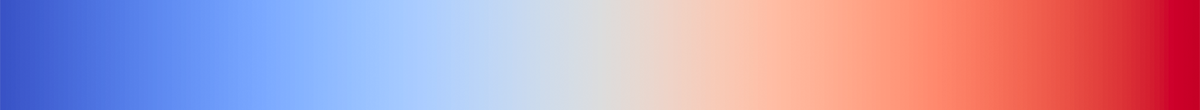
\includegraphics[width=.44\linewidth, height=5mm]{map-cool-to-warm} & 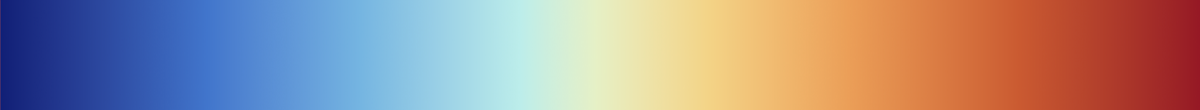
\includegraphics[width=.44\linewidth, height=5mm]{map-fast} \\
    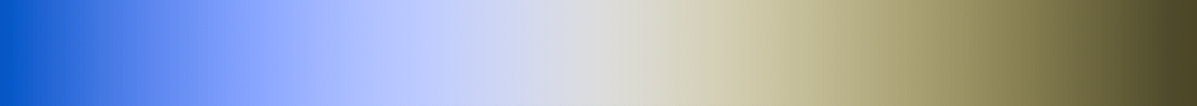
\includegraphics[width=.44\linewidth, height=5mm]{map-protanopia-cool-to-warm} & 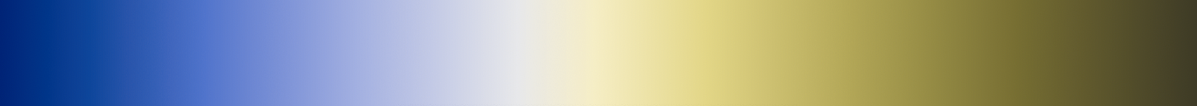
\includegraphics[width=.44\linewidth, height=5mm]{map-protanopia-fast} \\
    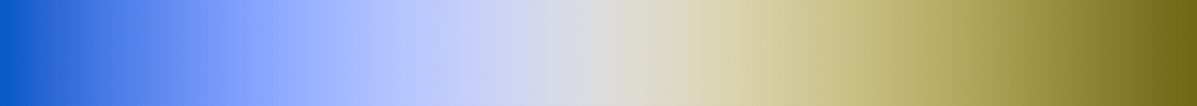
\includegraphics[width=.44\linewidth, height=5mm]{map-deurteranopia-cool-to-warm} & 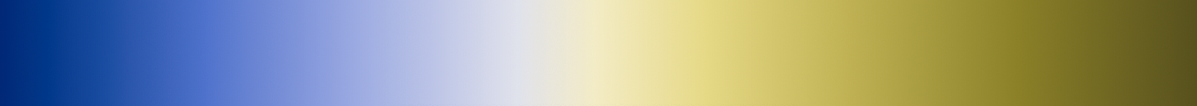
\includegraphics[width=.44\linewidth, height=5mm]{map-deurteranopia-fast}
  \end{tabular}
  \caption{
    Colorblindness simulation of \coolwarm (left) and \fast (right) colormaps.
    The top row is the original colors.
    The middle row is the colors simulated for protanopia.
    The bottom row is the colors simulated for deurteranopia.
  }
  \label{fig:colorblindness}
\end{figure}

\section{ACKNOWLEDGMENT}

The authors wish to thank the ParaView software development team at Kitware, Inc. for assisting in making these changes to the software. We also wish to thank those in the ParaView community who provided the necessary feedback to guide our designs. We also wish to acknowledge the contributions made by the Data Science at Scale, LANL~\cite{SciVisColor}, for their contributions and support for the underlying color research and Khairi Reda for help with namability evaluations of colormaps.

This work was supported in part by the U.S. Department of Energy (DOE) RAPIDS SciDAC project under contract number DE-AC05-00OR22725. This paper describes objective technical results and analysis. Any subjective views or opinions that might be expressed in the paper do not necessarily represent the views of the U.S. Department of Energy or the United States Government. This work was done in part at Sandia National Laboratories, which is a multi-mission laboratory managed and operated by National Technology and Engineering Solutions of Sandia, LLC, a wholly owned subsidiary of Honeywell International Inc., for the U.S. Department of Energy's National Nuclear Security Administration under contract DE-NA0003525.


\bibliographystyle{IEEEtran}
\bibliography{Fast_ParaView}

\begin{IEEEbiography}{Francesca Samsel}{\,}is a Research Scientist at the Texas Advanced Computing Center, University of Texas at Austin. She received an M.F.A. from the University of Washington and a B.F.A. from California College of Art. Prior to turning her attention to scientific visualization she taught sculpture and design in the Art Department of Fordham University at Marymount. Her research focuses on expanding the visual language used to encode scientific data as well as experimenting with forms of interactive and physicalized data. Contact her at fsamsel@tacc.utexas.edu.
\end{IEEEbiography}

\begin{IEEEbiography}{W. Alan Scott}{\,}is Sandia National Laboratories' ParaView Support Manager.  He received an MS degree in computer science from Utah State University in 1992, focusing on computer architectures, parallel processing, compiler design, and graphics.  His current interests include ParaView functionality and user experiences.  Contact him at wascott@sandia.gov.
\end{IEEEbiography}

\begin{IEEEbiography}{Kenneth Moreland,}{\,} with Oak Ridge National Laboratory, is a senior member of IEEE.
  He received MS and Ph.D. degrees in computer science from the University of New Mexico in 2000 and 2004, respectively.
  Dr. Moreland specializes in large-scale visualization and graphics and plays an active role in the development of several HPC products including ParaView, VTK, IceT, Catalyst, and VTK-m.
  His current interests include the design and development of visualization algorithms and systems to run on multi-core, many-core, and future-generation computer hardware.
  Contact him at morelandkd@ornl.gov.
\end{IEEEbiography}

\end{document}

